\documentclass[11pt]{beamer}

\usepackage{hyperref}

% Hey Nick!
% Percent sign is a comment
% \begin{frame} \end{frame} is a page on the presentation
% \section denotes a new section, \subsection new subsection, \subsubsection, etc (used for Table of Contents)
% \pause Things after \pause will only show on pressing space, return, or page down, etc.
% See: https://en.wikibooks.org/wiki/LaTeX/Presentations for more information :-)

\hypersetup{pdfstartview={Fit}}  % Fits the presentation to the window when first displayed.
\usetheme{Berlin}
\usecolortheme{beaver}
\beamertemplatenavigationsymbolsempty

%Gummi|065|=)
\title[Bitmap Indexes for Large Datasets]{\textbf{Using Bitmap Index for Interactive Exploration of Large Datasets}}
\subtitle{INFO3504 Presentation}
\author{Nick Armstrong \\
        Daniel Collis}
\titlegraphic{
\includegraphics[height=1cm]{usydlogo.png}}
\institute{University of Sydney}
\date{}
\subject{Computer Science}

\begin{document}

% Front page
\frame{\titlepage}

% Table of Contents
\begin{frame}
	\frametitle{Table of Contents}
	\tableofcontents
\end{frame}

\section[Bitmap Indexes]{Bitmap Indexes}

\begin{frame}
	\frametitle{Bitmap Indexes}
	
	Bitmap Indexes:
	\begin{itemize}
		\pause
		\item Are an old idea
		\pause
		\item Are efficient for big data and data warehouse solutions with read-only records
		\pause
		\item Do not reorder data, unlike some other algorithms
	\end{itemize}
\end{frame}

\subsection[Bitmap Indexes]{What Are They?}
\begin{frame}
	\frametitle{What Are They?}
	
	For those who weren't in last week's lecture, they \pause are a way to represent records and fields as a grid (essentially).
	
	\pause
	\begin{exampleblock}{Just imagine...}
		Imagine a table, with a bunch of records ($R_x$) and an enumeration ($A_x = \{1, 2, 3\}$):
		
		\pause
		\begin{tabular}{r|c|c|c|c}
				& \textbf{Value} & $A_1$ & $A_2$ & $A_3$ \\ \hline
			$R_1$ & $3$	& 	& 	& \\
			$R_2$ & $1$	& 	& 	& \\
			$R_3$ & $1$	& 	& 	& \\
			$R_4$ & $2$	& 	& 	& \\
			$R_5$ & $3$	& 	& 	& 
		\end{tabular}
	\end{exampleblock}
\end{frame}

\begin{frame}
	\frametitle{What Are They?}
	
	For those who weren't in last week's lecture, they are a way to represent records and fields as a grid (essentially).
	
	\begin{exampleblock}{Just imagine...}
		Imagine a table, with a bunch of records ($R_x$) and an enumeration ($A_x = \{1, 2, 3\}$):
		
		\begin{tabular}{r|c|c|c|c}
				& \textbf{Value} & $A_1$ & $A_2$ & $A_3$ \\ \hline
			$R_1$ & $3$	& $0$	& $0$	& $1$ \\
			$R_2$ & $1$	& $1$	& $0$	& $0$ \\
			$R_3$ & $1$	& $1$	& $0$	& $0$ \\
			$R_4$ & $2$	& $0$	& $1$	& $0$ \\
			$R_5$ & $3$	& $0$	& $0$	& $1$ 
		\end{tabular}
	\end{exampleblock}
\end{frame}

\begin{frame}
	\frametitle{What Are They?}
	
	The example table mentioned before can become really really big with multiple attributes and multiple rows.
	\pause
	\begin{exampleblock}{Lot's of attributes!}
		It could look something like this:
		
		\begin{columns}[c]
			\column{.4\textwidth}
			\begin{tabular}{r|c|c|c|c}
					& \textbf{Value} & $A_1$ & $A_2$ & $A_3$ \\ \hline
				$R_1$ & $3$	& $0$	& $0$	& $1$ \\
				$R_2$ & $1$	& $1$	& $0$	& $0$ \\
				$R_3$ & $1$	& $1$	& $0$	& $0$ \\
				$R_4$ & $2$	& $0$	& $1$	& $0$ \\
				$R_5$ & $3$	& $0$	& $0$	& $1$ 
			\end{tabular}
			\column{.4\textwidth}
			\begin{tabular}{r|c|c|c|c}
					& \textbf{Value} & $B_1$ & $B_2$ & $B_3$ \\ \hline
				$R_1$ & $1$	& $1$	& $0$	& $0$ \\
				$R_2$ & $1$	& $1$	& $0$	& $0$ \\
				$R_3$ & $3$	& $0$	& $0$	& $1$ \\
				$R_4$ & $2$	& $0$	& $1$	& $0$ \\
				$R_5$ & $3$	& $0$	& $0$	& $1$ 
			\end{tabular}
		\end{columns}	
	\end{exampleblock}
	
	\pause
	How to determine if a record matches multiple attributes? Use a bitwise-AND!
	
	\pause
	This is quite a quick and efficient operation.
\end{frame}

\section[Bitmap Compression]{Bitmap Compression}
\begin{frame}
	\frametitle{Bitmap Compression}
	
	Bitmap Indexes are great, efficient, and all. But, they can become very large!
	\pause
	The researchers of this paper had two data samples:
	\begin{itemize}
		\pause
		\item $1.6$ GiB
		\pause
		\item $30$ GiB
	\end{itemize}
	
	\pause
	Storing these in a typical database with a \texttt{Bitmap Index} took $3\times$ the size, similar to when using a \texttt{B-Tree Index} \pause $=$ Not ideal!
\end{frame}

\begin{frame}
	\frametitle{Bitmap Compression}
	
	What can we do?
	\begin{itemize}
		\pause
		\item Run-Length Encoding
		\pause
		\item Word-Aligned Hybrid (WAH)
	\end{itemize}
\end{frame}

\subsection[Word-Aligned Hybrid]{Word-Aligned Hybrid}
\begin{frame}
	\frametitle{Word-Aligned Hybrid (WAH)}
	
	A patent exists for it:
	\begin{columns}[c]
		\column{4cm}
		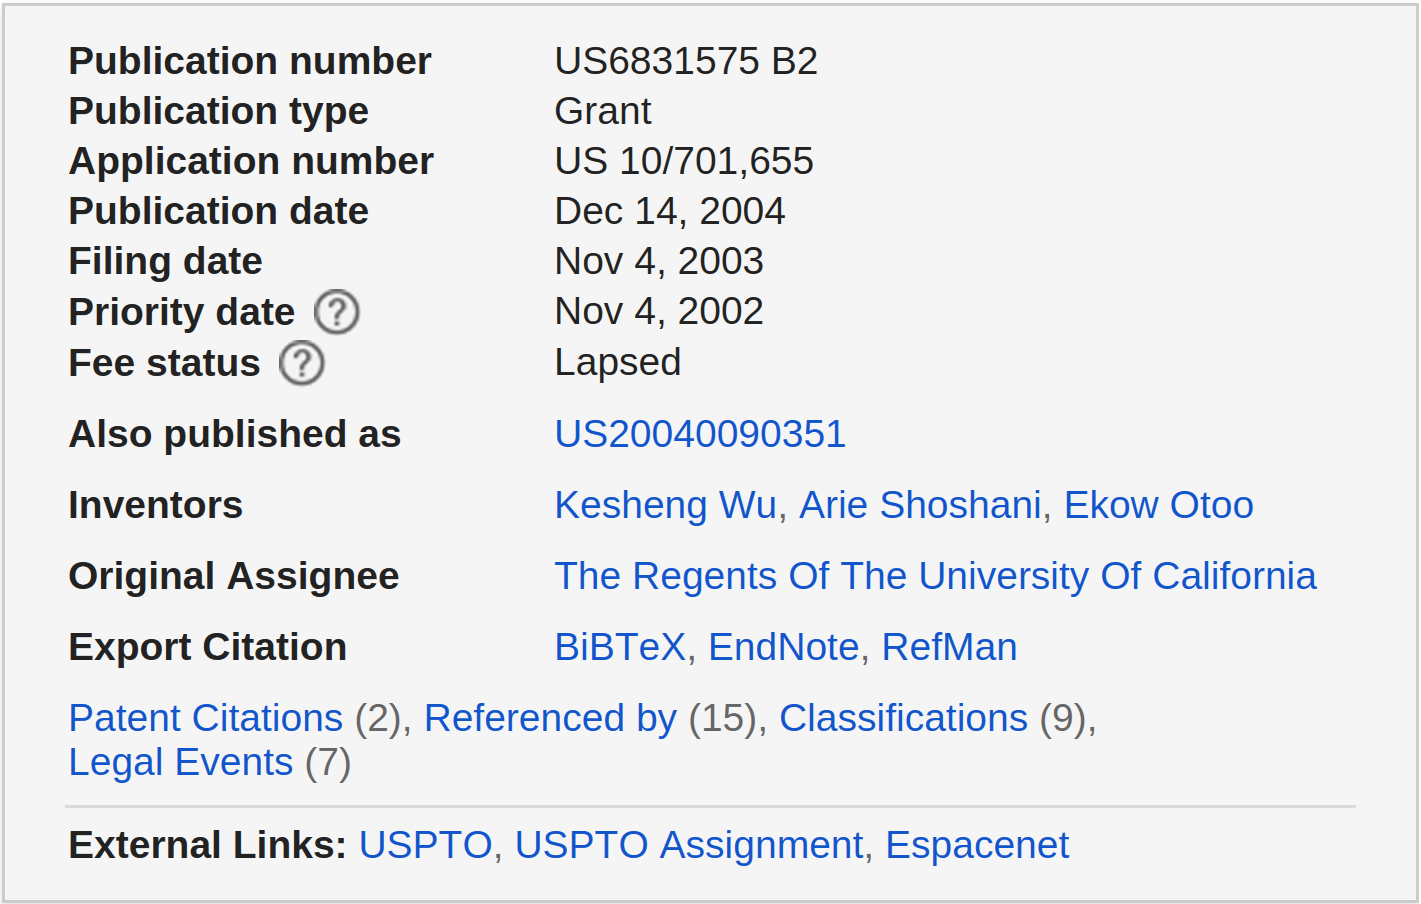
\includegraphics[height=3cm]{patent.png}\footnotemark
		\column{6cm}
		\pause
		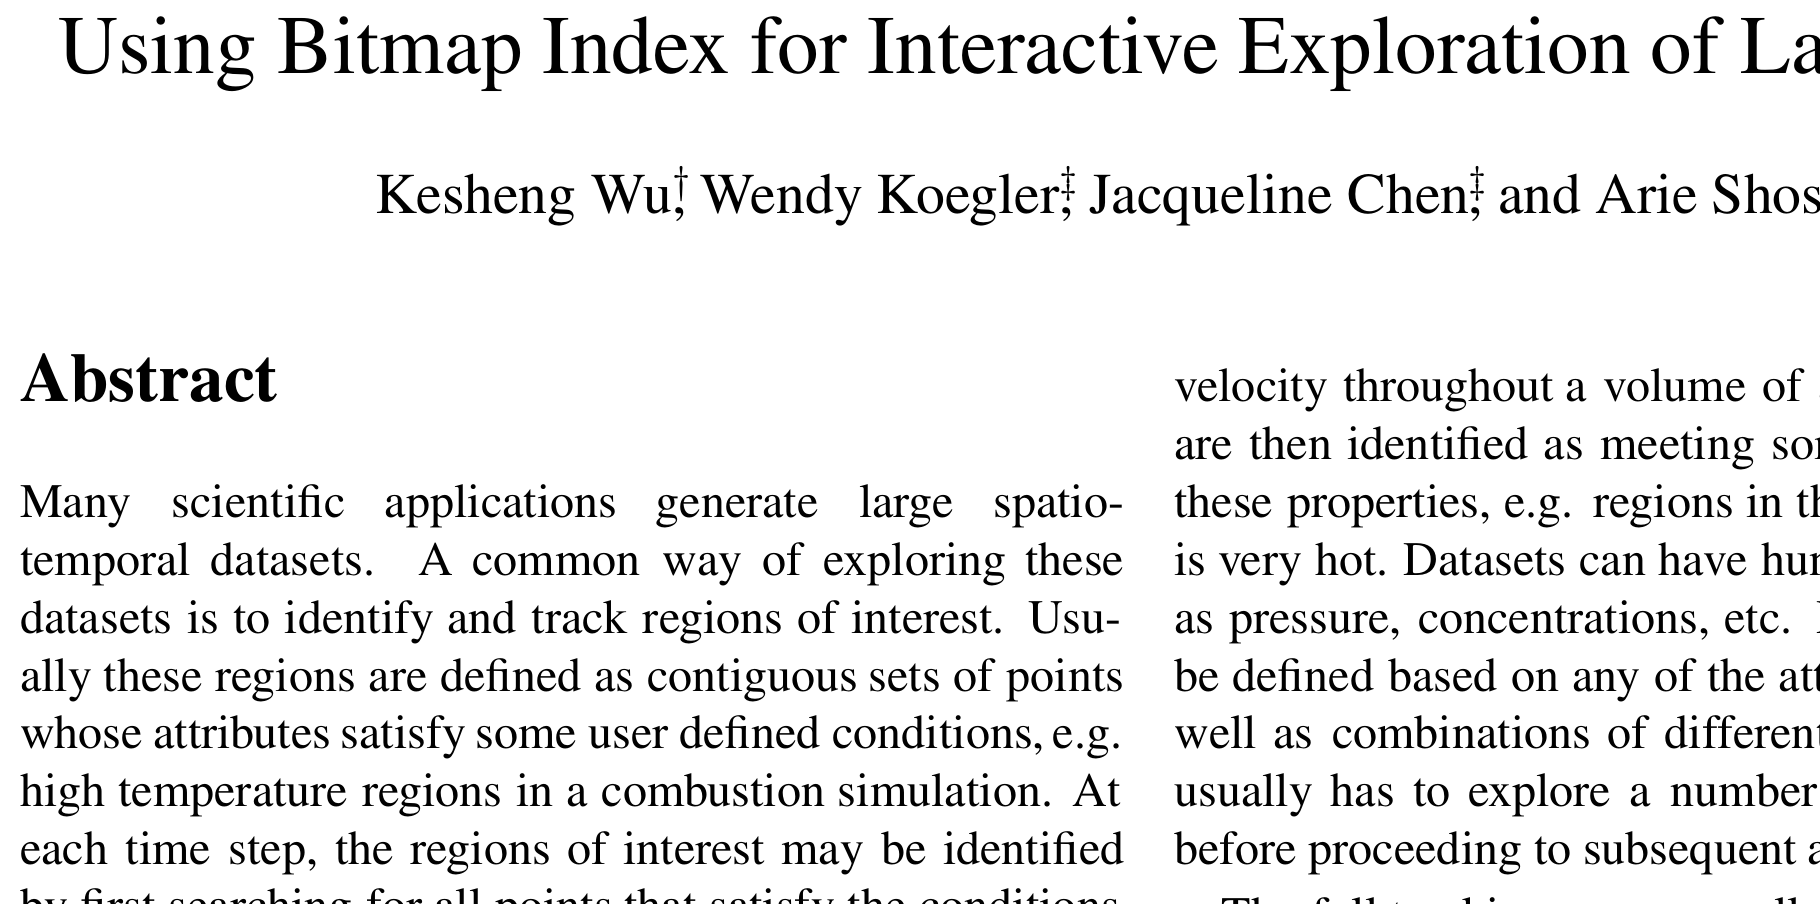
\includegraphics[height=3cm]{paper2.png}\footnotemark
	\end{columns}
	
	\footnotetext[1]{\url{https://www.google.com/patents/US6831575}}
	\footnotetext[2]{Blah}
\end{frame}

\subsubsection[Word-Aligned Hybrid]{What Is It?}
\begin{frame}
	\frametitle{What Exactly Is It?}
	
	Differs from Run Length Encoding in \textbf{two} major ways:
	\begin{itemize}
		\pause
		\item It only records long groups of $0$s or $1$s using Run Length Encoding (the short groups are represented \textit{literally})
		\pause
		\item It requires groups of a certain size so that operations on the compressed data are efficient
	\end{itemize}
\end{frame}

\subsubsection[Word-Aligned Hybrid]{How Does It Work?}
\begin{frame}
	\frametitle{How Does It Work?}
	
	\begin{block}{Understand: What Is A Fill?}
		A group of consecutive identical bits. 
		
		A fill with only $0$s is called a $0$-fill and a fill with only $1$s is called a $1$-fill.
	\end{block}
	\begin{block}{Understand: Word-Size?}
		The word size is dependent on the computer architecture. On x86 machines (32-bit), the word size is 32-bits. On x86\_64/amd64 machines, the word size is 64-bits.
	\end{block}
\end{frame}

\begin{frame}
	\frametitle{How Does It Work?}
	
	\begin{enumerate}
		\item Split the bitmap index into multiple rows of size: $\texttt{word-length}- 1$
		\item If the row is \textbf{NOT} entirely made up of either $1$s or $0$s (i.e. not a 0-fill or a 1-fill), then keep as is (\textit{literal}) and prefix row with a $0$
		\item Otherwise, determine how many following rows are also fill rows. Prefix the row with a $1$ (fill bit), mark the second bit with the type of bit that is to be filled, then the rest of the bits are how many subsequent rows also match this criteria
	\end{enumerate}
	
	\pause
	Who understands all of that?
\end{frame}

\begin{frame}
	\frametitle{How Does It Work?}
	
	Let's go back to our example:
	\begin{exampleblock}{Just imagine...}
		Imagine a table, with a bunch of records ($R_x$) and an enumeration ($A_x = \{1, 2, 3\}$):
	
		\begin{tabular}{r|c|c|c|c}
				& \textbf{Value} & $A_1$ & $A_2$ & $A_3$ \\ \hline
			$R_1$ & $3$	& $0$	& $0$	& $1$ \\
			$R_2$ & $1$	& $1$	& $0$	& $0$ \\
			$R_3$ & $1$	& $1$	& $0$	& $0$ \\
			$R_4$ & $2$	& $0$	& $1$	& $0$ \\
			$R_5$ & $3$	& $0$	& $0$	& $1$ 
		\end{tabular}
	\end{exampleblock}

	\pause
	Let's perform WAH on $A_1$. \pause Let's turn it on its side: $A_1 = \texttt{01100}$
\end{frame}

\begin{frame}
	\frametitle{How Does It Work?}
	
	Preamble:
	\begin{itemize}
		\item Let's turn it on its side: $A_1 = \texttt{01100}$
		\item Assume that our word size is $16$ bits.
		\item Assume that there are $60$ tuples (i.e. $R_1, R_2, \dotsm, R_{31}, R_{32}$)
	\end{itemize}
	
	\pause
	\begin{tabular}{rl}
		$A_1 =$	& \texttt{011001001011010} \\
				& \texttt{000000000000000} \\
				& \texttt{000000000000000} \\
				& \texttt{100110110100101}
	\end{tabular}
	
	\pause
	Result from applying WAH: \\
	\begin{tabular}{rll}
		$A_1 =$	& \texttt{0} 	& \texttt{011001001011010} \\
		\pause
				& \texttt{10} 	& \texttt{00000000000010} \\
		\pause
				& \texttt{0} 	& \texttt{100110110100101}
	\end{tabular}
\end{frame}

\begin{frame}
	\frametitle{Example From Paper}
	
	\begin{columns}[c]
		\column{.5\textwidth}
		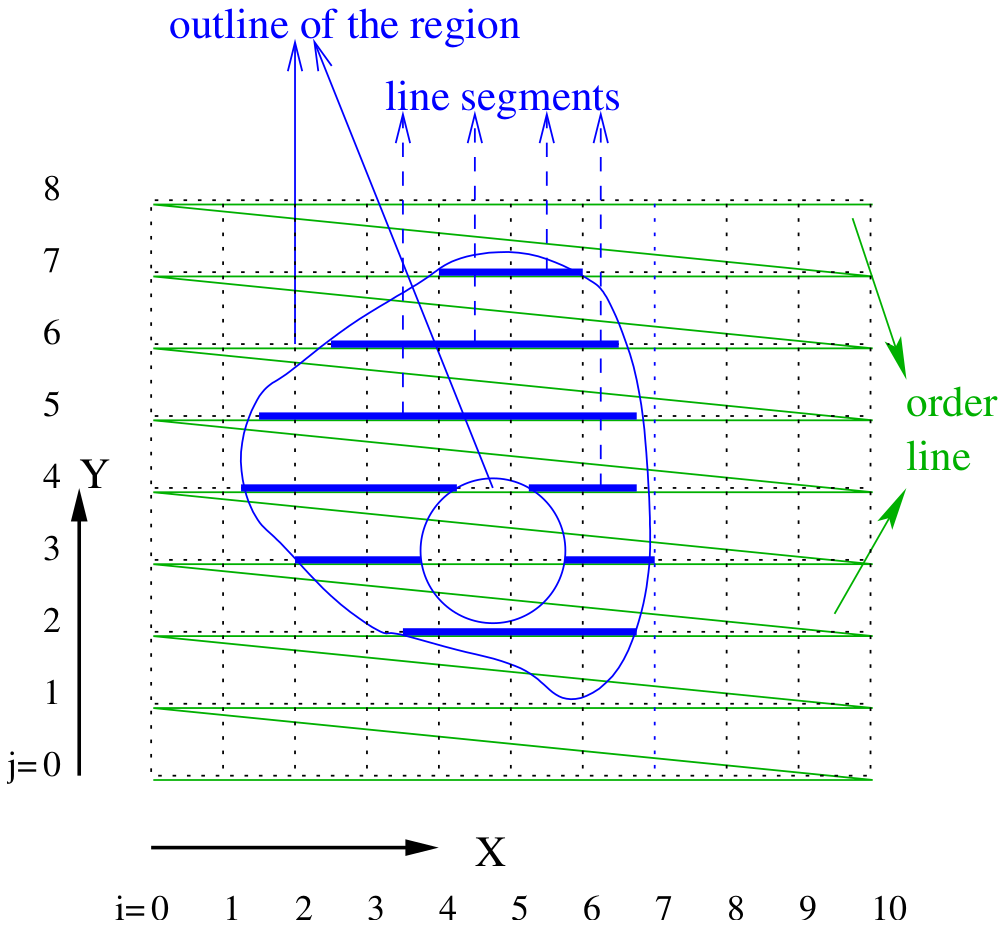
\includegraphics[height=5cm]{example_grid.png}
		\column{.5\textwidth}
		\pause
		Run-Length Encoding: $26 \times 0$, $3 \times 1$, $6 \times 0$, $2 \times 1$, $2 \times 0$, $1 \times 1$, $6 \times 0$, $3 \times 1$, $1 \times 0$, $1 \times 1$, $6 \times 0$, $5 \times 1$, $7 \times 0$, $4 \times 1$, $8 \times 0$, $3 \times 1$, $15 \times 0$
		
		\pause
		WAH Encoding (in hex): \texttt{0000001C} \texttt{0640E81F} \texttt{00F00E00} \texttt{00000000}
	\end{columns}
\end{frame}

\subsubsection[Word-Aligned Hybrid]{Versus Run Length Encoding}
\begin{frame}
	\frametitle{Versus Run Length Encoding}
	
	\begin{itemize}
		\item In theory, it is not as compressible as Run Length Encoding. \pause But in practice, it takes less space than the Run Length Encoding scheme, especially if many of the groups are small
		
		\pause
		\item Logical operations on WAH compressed bitmaps can work \textit{directly} on the compressed data and \textit{generate compressed answers}. Because of this, the time to perform these operations is proportional to the sizes (bytes) of the bitmaps involved.
		
		\pause
		\item We can generate bitmap indices efficiently. Using WAH compression, it is possible to only insert bits that are $1$ when creating a bitmap index. In practice, generating a bitmap index has the computational complexity of $O(N \text{log}(b))$ (where $b$ is number of bitmaps generated), compared to generating an uncompressed bitmap index: $O(Nb)$ (significantly worse).
	\end{itemize}
\end{frame}

% End of Daniel's Part

\section[Region Growing]{Region Growing}

\section[Region Tracking]{Region Tracking}

\section[Finish]{Finish}

\begin{frame}
	\Large{Thanks!}
\end{frame}

\end{document}
